
\subsection{L'Application Checkers}

l'application Checkers (principe), décompilation, un bytecode obscure
dex2jar, jd-gui, correction des erreurs, éclaircissement du code, une archi mvc.
Fonctionnement de l'appli en interne
\subsubsection{Principe}
\begin{figure}[hp]
	      \begin{center}
		\fbox{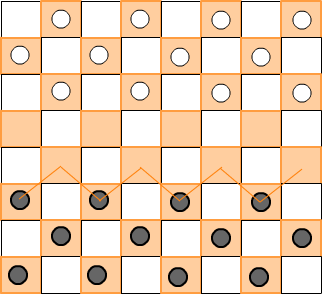
\includegraphics[scale=0.5]{principe}}
	      \end{center}
	\legend{Principe}
\end{figure}
Le jeu est composé de 8 cases sur 8, c’est-à-dire 4 cases en moins que le jeu de dame classique.  Se joue en deux modes : utilisateur contre ordinateur ou utilisateur contre utilisateur.\\
Un joueur peut choisir une couleur (des pions/dames noires ou des pions/dames blanche).  Le jeu est initialement constitué de 3 lignes de 4 pions espacés d’une case. Chaque pion/dame peut se déplacer en diagonale. 
Un pion se transforme en une dame (K) lorsqu’il arrive à la dernière ligne du camp de l’adversaire. Une dame ou un pion peut faire une prise en faisant un déplacement en diagonal. Mais une dame possède l’avantage de traverser plusieurs lignes vide.\\
Un joueur est désigné gagnant si l’adversaire ne possède plus de dames ou de pions. 
\subsubsection{Décompilation et analyse du code}

\newpage
\subsubsection{Architecture}
Dans un point de vue général, le développeur du jeu Checkers a adopté une architecture MVC. Ce qui nous a beaucoup aidé à determiner les différentes 
classes. 
\begin{figure}[hp]
	      \begin{center}
		\fbox{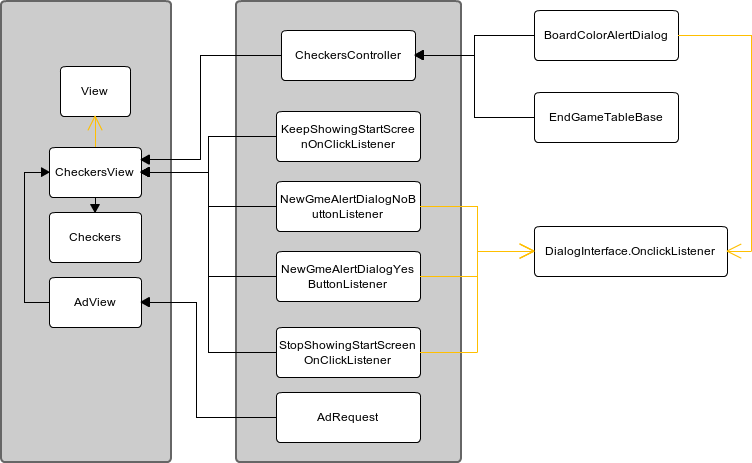
\includegraphics[scale=0.6]{archi}}
	      \end{center}
	\legend{architecture}
\end{figure}
La classe Checkers est la classe principale de l’application.
La classe CherckersView (b.smali) hérite de la classe android.view.View qui gére les vues de l’application. La classe AdView gère la vue pour la publicité.
CheckersController (a.smali) est le controleur principal de l’application. Les classes KeepShowingStartScreenOnclickListener (e.smali), NewGameAlertDialogNoButtonListener (d.smali), NewGameAlertDialogYesButtonListener (c.smali) et StopShowingStartScreenOnclickListener (f.smali) implémente l'interface DialogInterface.OnclickListener sont les classes qui gère les clics.
AdRequest est la classe qui est responsable du chargement de la publicité.
